\begin{tikzpicture}[
  x=1cm,
  y=1cm,
  panel/.style={font=\sffamily\bfseries\small, anchor=north west, fill=white,
    fill opacity=0.86, text opacity=1, inner sep=2pt},
  %label/.style={font=\sffamily\bfseries\small, align=center},
  label/.style={font=\sffamily\small, align=center},
  note/.style={font=\sffamily\scriptsize, align=center, text=black!70,
    text width=0.27\linewidth},
]

% Panel sizes and positions can be tuned directly from here.
\def\adndpw{0.29\linewidth}
\def\yimage{0}
\def\ylabel{-2.55}
\def\ynote{-3.35}

\node[inner sep=0pt] (pt10c) at (-4.25,\yimage)
  {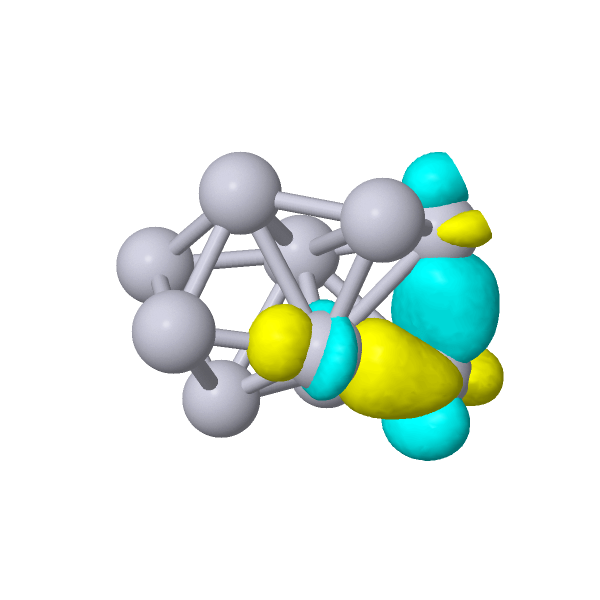
\includegraphics[width=\adndpw]{adndp_pt10_3c_600.png}};
\node[inner sep=0pt] (pt5geptpt) at (0,\yimage)
  {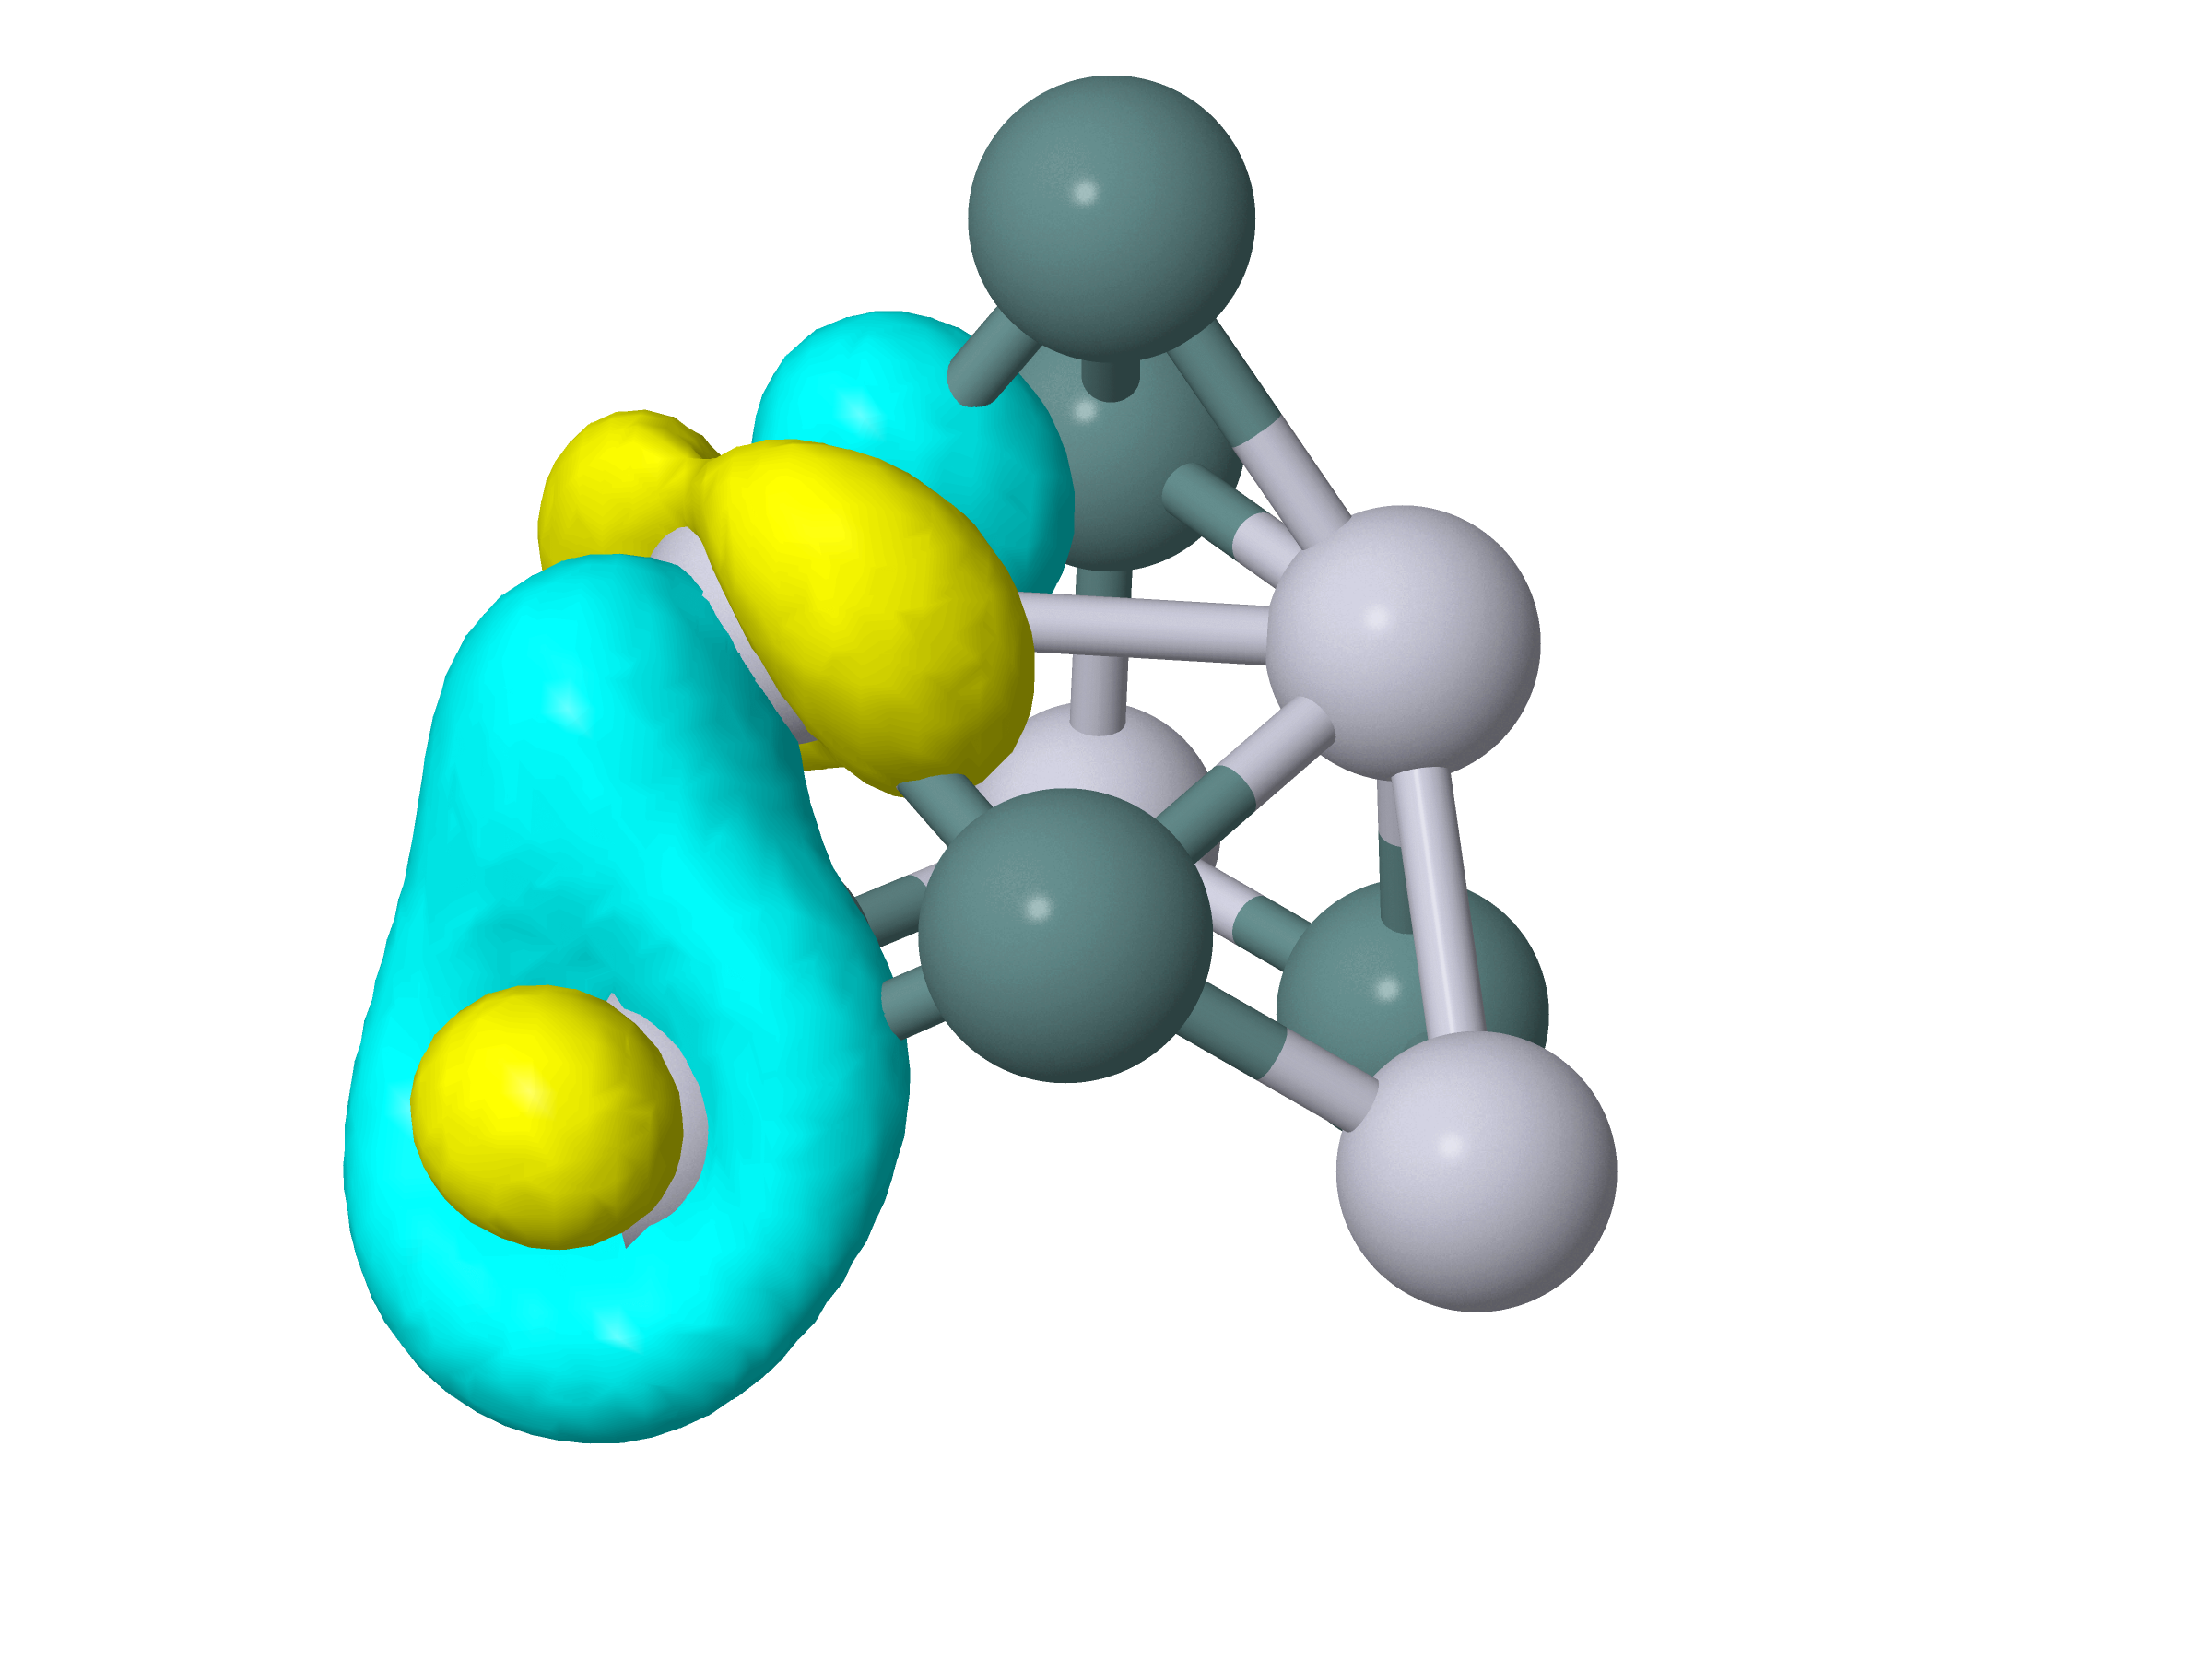
\includegraphics[width=\adndpw]{Pt-Pt_orbital25.png}};
\node[inner sep=0pt] (pt5geptge) at (4.25,\yimage)
  {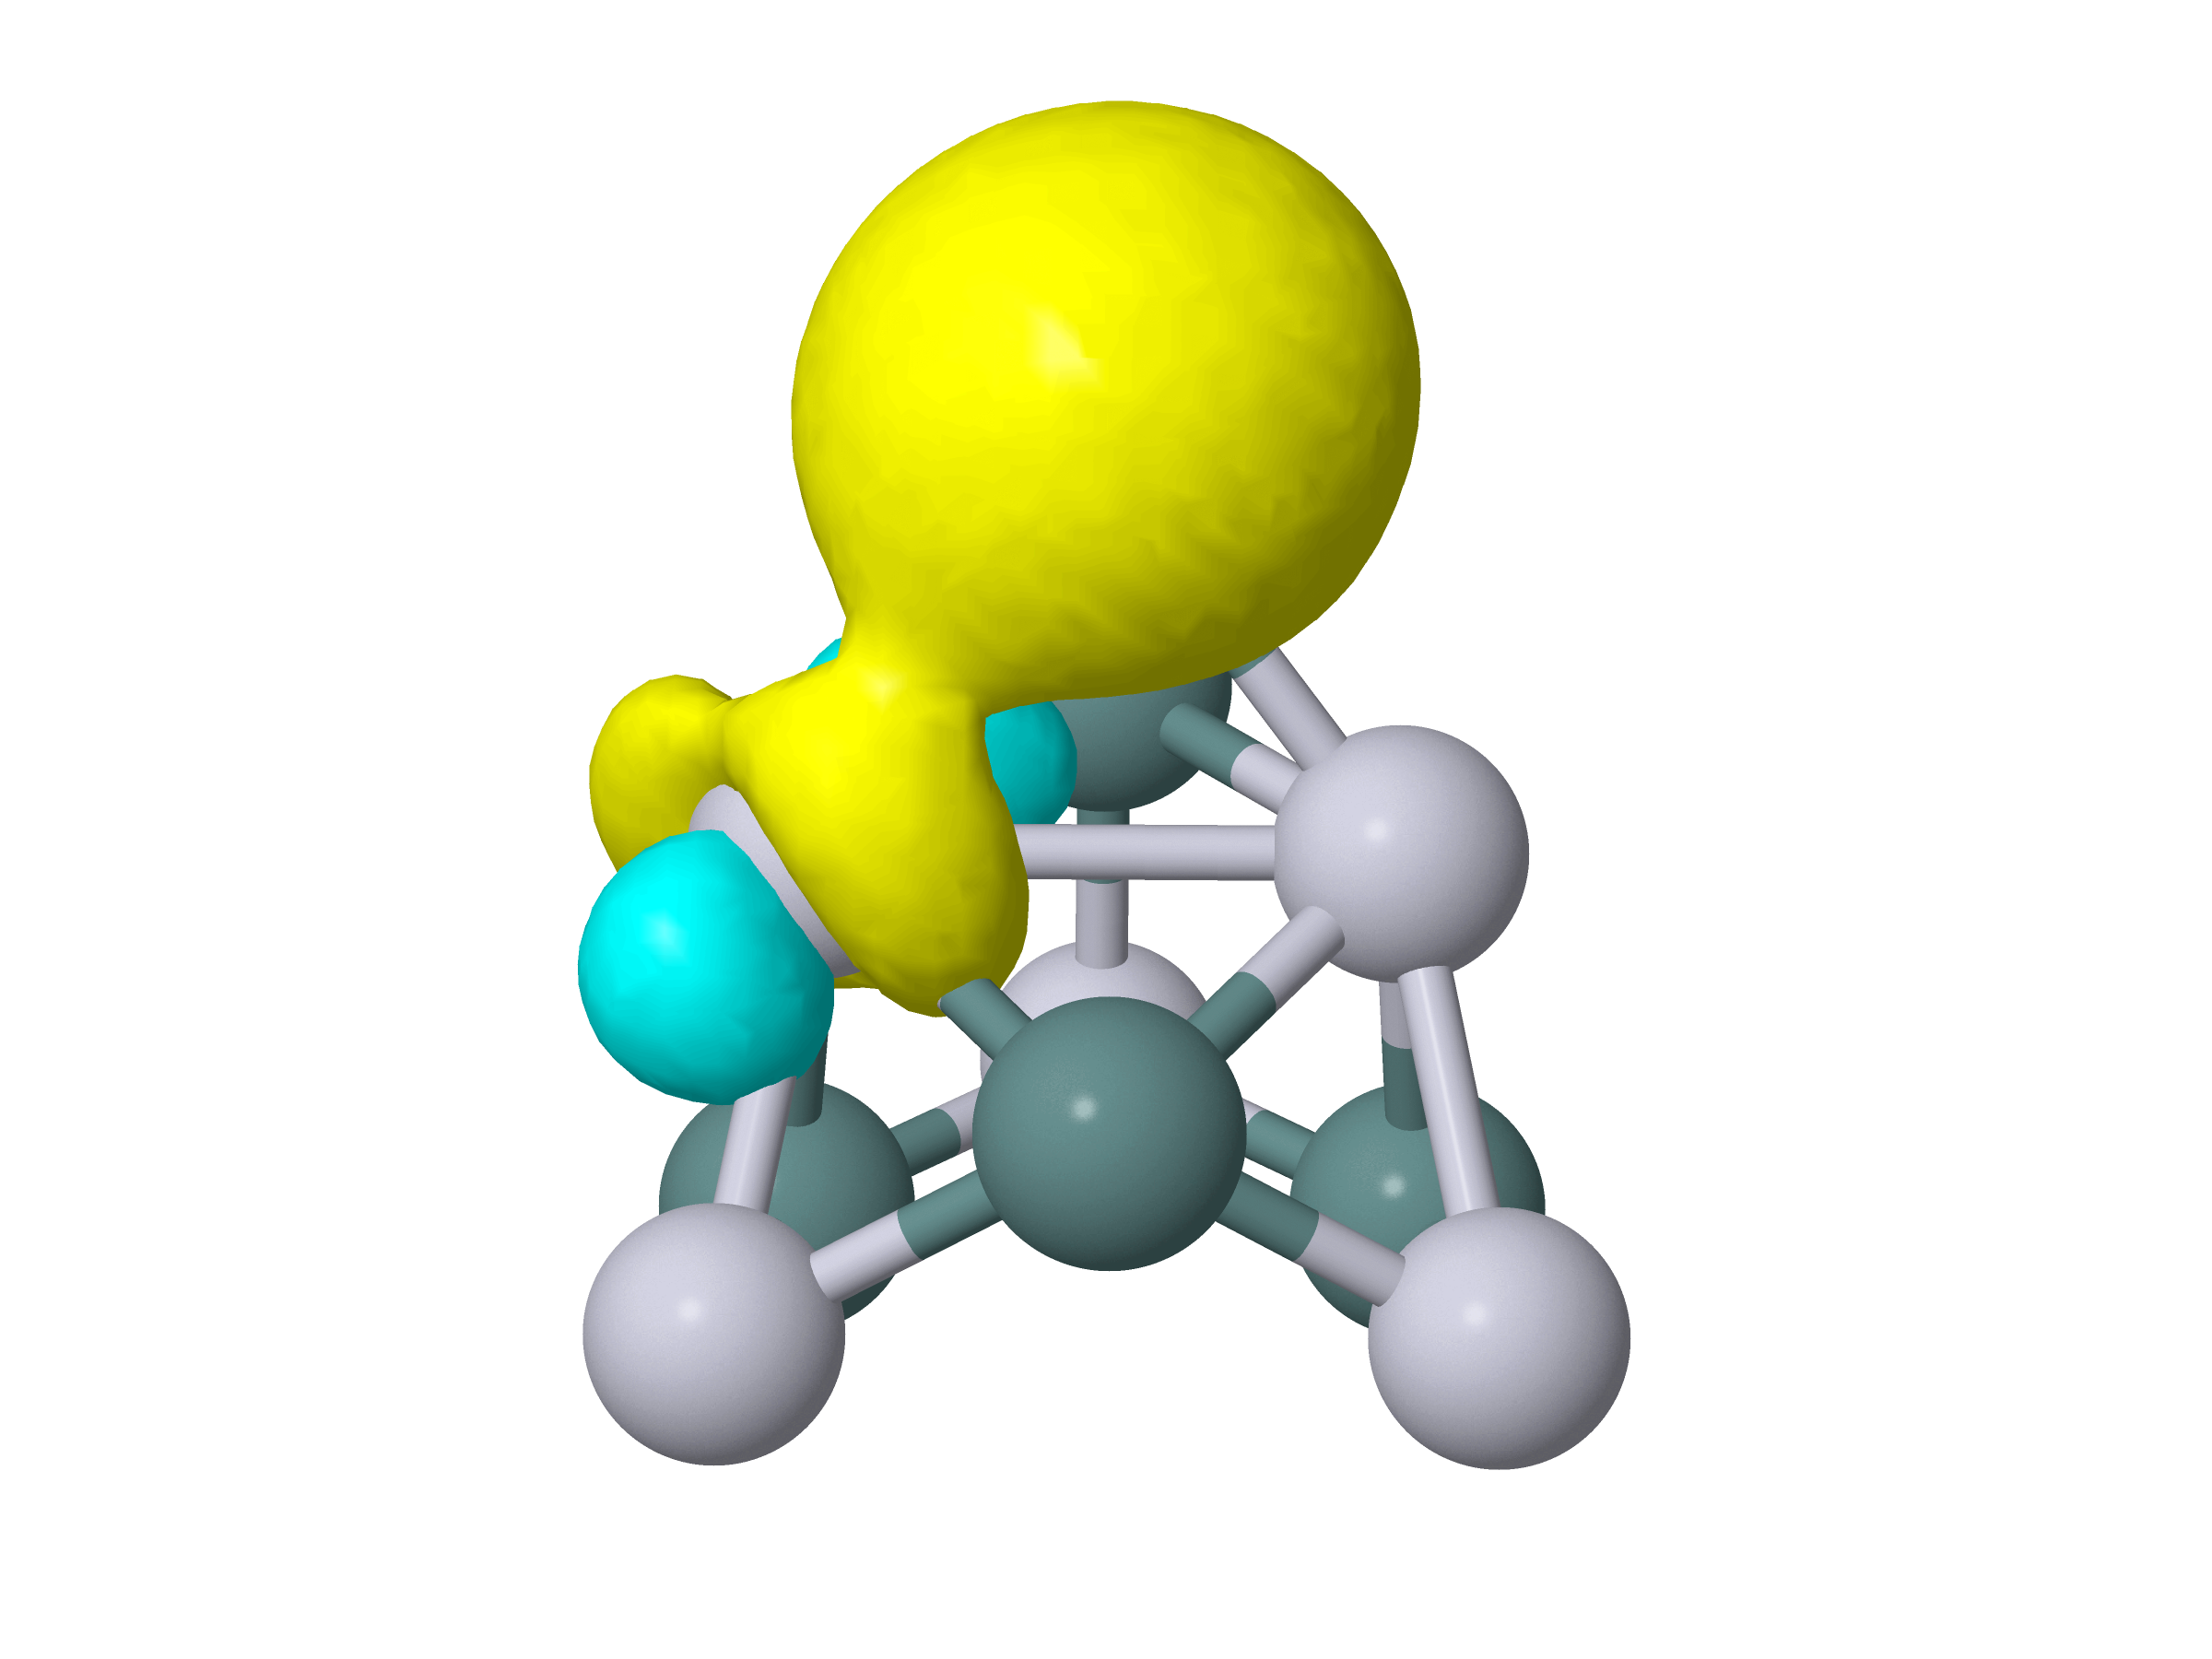
\includegraphics[width=\adndpw]{Pt-Ge_orbital27.png}};

\node[panel] at ([xshift=-1.75cm,yshift=1.82cm]pt10c.center) {(a)};
\node[panel] at ([xshift=-1.75cm,yshift=1.82cm]pt5geptpt.center) {(b)};
\node[panel] at ([xshift=-1.75cm,yshift=1.82cm]pt5geptge.center) {(c)};

\node[label] at (-4.25,\ylabel) {\ce{Pt10^{der}}};
\node[note] at (-4.25,\ynote) {representative 3c element};
\node[label] at (0,\ylabel) {\ce{Pt5Ge5^{der}}};
\node[note] at (0,\ynote) {Pt--Pt 2c--2e element};
\node[label] at (4.25,\ylabel) {\ce{Pt5Ge5^{der}}};
\node[note] at (4.25,\ynote) {Pt--Ge 2c--2e element};

\end{tikzpicture}
